\documentclass[11pt]{article}\usepackage[]{graphicx}\usepackage[]{xcolor}
% maxwidth is the original width if it is less than linewidth
% otherwise use linewidth (to make sure the graphics do not exceed the margin)
\makeatletter
\def\maxwidth{ %
  \ifdim\Gin@nat@width>\linewidth
    \linewidth
  \else
    \Gin@nat@width
  \fi
}
\makeatother

\definecolor{fgcolor}{rgb}{0.345, 0.345, 0.345}
\newcommand{\hlnum}[1]{\textcolor[rgb]{0.686,0.059,0.569}{#1}}%
\newcommand{\hlstr}[1]{\textcolor[rgb]{0.192,0.494,0.8}{#1}}%
\newcommand{\hlcom}[1]{\textcolor[rgb]{0.678,0.584,0.686}{\textit{#1}}}%
\newcommand{\hlopt}[1]{\textcolor[rgb]{0,0,0}{#1}}%
\newcommand{\hlstd}[1]{\textcolor[rgb]{0.345,0.345,0.345}{#1}}%
\newcommand{\hlkwa}[1]{\textcolor[rgb]{0.161,0.373,0.58}{\textbf{#1}}}%
\newcommand{\hlkwb}[1]{\textcolor[rgb]{0.69,0.353,0.396}{#1}}%
\newcommand{\hlkwc}[1]{\textcolor[rgb]{0.333,0.667,0.333}{#1}}%
\newcommand{\hlkwd}[1]{\textcolor[rgb]{0.737,0.353,0.396}{\textbf{#1}}}%
\let\hlipl\hlkwb

\usepackage{framed}
\makeatletter
\newenvironment{kframe}{%
 \def\at@end@of@kframe{}%
 \ifinner\ifhmode%
  \def\at@end@of@kframe{\end{minipage}}%
  \begin{minipage}{\columnwidth}%
 \fi\fi%
 \def\FrameCommand##1{\hskip\@totalleftmargin \hskip-\fboxsep
 \colorbox{shadecolor}{##1}\hskip-\fboxsep
     % There is no \\@totalrightmargin, so:
     \hskip-\linewidth \hskip-\@totalleftmargin \hskip\columnwidth}%
 \MakeFramed {\advance\hsize-\width
   \@totalleftmargin\z@ \linewidth\hsize
   \@setminipage}}%
 {\par\unskip\endMakeFramed%
 \at@end@of@kframe}
\makeatother

\definecolor{shadecolor}{rgb}{.97, .97, .97}
\definecolor{messagecolor}{rgb}{0, 0, 0}
\definecolor{warningcolor}{rgb}{1, 0, 1}
\definecolor{errorcolor}{rgb}{1, 0, 0}
\newenvironment{knitrout}{}{} % an empty environment to be redefined in TeX

\usepackage{alltt}
%\usepackage{fullpage}
\usepackage{graphicx}
\usepackage[utf8]{inputenc}
\usepackage{amsmath}
\usepackage{graphics}
\usepackage{float}
\usepackage{xcolor}
\usepackage{geometry}
\usepackage{tikz}
\usetikzlibrary{shapes, arrows}
\usepackage[utf8]{inputenc}
\usepackage{amsmath}
\usepackage{graphics}
\usepackage{xcolor}
\usepackage{enumitem}
\usepackage{hyperref}
\usepackage{longtable}
\usepackage{array}
\numberwithin{equation}{section}
\numberwithin{table}{section}
\newlist{bracketedromanenum}{enumerate}{1}
\setlist[bracketedromanenum]{
	label={(\roman*)},
	ref={\roman*},
	itemsep=0.5em,
	topsep=0.5em
}
\IfFileExists{upquote.sty}{\usepackage{upquote}}{}
\begin{document}
	\begin{titlepage}
		
		\begin{center}
			
			
\includegraphics[width=0.3\textwidth]{UoN_Logo.png}\\
			\vspace{0.3cm}
			THE UNIVERSITY OF NAIROBI\\
			FACULTY OF SCIENCE AND TECHNOLOGY\\
			DEPARTMENT OF MATHEMATICS\\
			\vspace{0.5cm}
			\underline{	STA : 420 PROJECT IN STATISTICS}
			\vspace{0.7cm}
			
			\textbf{Application of Multiple Linear Regression Model in Modelling Depression Among caregivers in a Rural Setting}
			
			\vspace{0.5cm}
			BY:\\
			
			BEVERLY KIND               : \hspace{0.2cm}    I63/4240/2019\\
			\vspace{0.5cm}
			WAMBUA CHARLES             : \hspace{0.2cm}    I63/4248/2019\\
				
			\vspace{0.5cm}
			ODHIAMBO KENNEDY           : \hspace{0.2cm}    I63/4282/2019\\
			\vspace{0.5cm}
			NYAENYA DOMINIC            : \hspace{0.2cm}    I63/4261/2019\\
			\vspace{0.5cm}
			 PETER DOKTA               : \hspace{0.2cm}    I63/136668/2019\\
			\vspace{0.7cm}
			\textbf{SUPERVISOR}\\
			\vspace{0.2cm}
			DR. LYDIA ADHIAMBO MUSIGA
			
			\vspace{0.6cm}
			Submitted in partial fulfillment of the requirements for the award of the degree in Bachelor of Science Statistics\\
			\vspace{0.3cm}
			MAY 2023
			
			
		\end{center}
	\end{titlepage}
	\pagenumbering{roman}
	\subsection{Declaration}
	\noindent We declare that this research project is our original work and has not been presented in any institution for any award or conferment of any degree.\\\\
	
	\begin{tabular}{l c r }
		\vspace{0.5cm}
		\noindent
		\textbf{NAME} & \textbf{REG. NO.} & \textbf{SIGNATURE} \\
		\vspace{0.5cm}
		ODHIAMBO KENNEDY OWINO & I63/4282/2019 & \dotfill \\
		\vspace{0.5cm}
		APONDI BEVERLY KIND & I63/4240/2019 & \dotfill  \\
		\vspace{0.5cm}
		CHARLES WAMBUA & I63/4248/2019 & \dotfill \\
		\vspace{0.5cm}
		PETER DOKTA & I63/136668/2019 & \dotfill \\
		\vspace{0.5cm}
		NYAENYA DOMINIC & I63/4261/2019 & \dotfill \\
	\end{tabular}
	
	\noindent This project has been submitted for examination with my approval as the University Supervisor.\\
	
	\vspace{1cm}
	\noindent \textbf{DR. LYDIA ADHIAMBO MUSIGA}\\
	
	\vspace{0.5cm}
	
	\noindent Signed: \dotfill Date: \dotfill \\
	
	\noindent SENIOR LECTURER\\
	DEPARTMENT OF MATHEMATICS, UNIVERSITY OF NAIROBI
	
	\newpage
	
	\subsection{Dedication}
	
	We dedicate this project to our parents, lecturers, relatives, and friends for their steadfast support during our university journey.
	
	\newpage
	
	\subsection{Acknowledgment}
	We dedicate this project to our parents, lecturers, relatives and friends for their We wish to thank everyone who helped in diverse ways with ideas, insights, research materials and software(s) exploration for this project.
	
	\noindent We are very grateful to the Almighty God for His direction and the gift of good health that has enabled us to undertake this initiative. We would like to express our heartfelt gratitude to Dr. Musiga (PhD) (Lecturer, University of Nairobi,School of Mathematics) and Dr. James Katende (Lecturer, University of Nairobi,School of Mathematics) for their unflinching support and help during this project.\\
	Furthermore, we are grateful to Dr. T.K Kamanu (PhD,CPA) (Bio-informatics Lecturer, University of Nairobi, School of Mathematics) for his active participation in teaching us computational statistics. The skills he taught us and the crucial insights he provided made this piece possible with reasonable ease. 
	\newpage
\tableofcontents
	\newpage
	\subsection{Abbreviations and Acronyms}
	\textbf{PHQ-9} - Patient Health Questionnaire-9 \\\\
	\textbf{VIF} - Variance Inflation Factor\\\\
	\textbf{SST} - Total sum of squares \\\\
	\textbf{$SS_{R}$} - Regression sum of squares\\\\
	\textbf{SSE} - Sum squares of residuals \\\\
	\textbf{ANOVA} - Analysis of variance\\\\
	\textbf{ACF}- Autocorrelation function 
	
	\newpage
	
	\subsection{Definition of Terms}
	\begin{itemize}
		\item  Multiple linear regression- is a statistical technique that uses several explanatory variables to predict the outcome of a response variable.
		\item Independent/predictor variables - Variables that are manipulated or changed to measure to the effect of that change on the outcome variable.
		\item Dependent/response variables -variables whose variation is being studied
		
		
	\end{itemize}
	
	\newpage
	\subsection{Abstract}
Support for cancer patients from their caregivers is crucial in terms of logistical, emotional, and physical care. However, the difficulties they encounter in rural areas can raise their vulnerability to depression. This abstract seeks to present a succinct overview of the incidence, contributing factors, and effects of depression in rural carers of cancer patients.\\
A comprehensive literature review was conducted, focusing on studies published between 2009 and 2023. Relevant databases including PubMed, PsycINFO, and Google Scholar were searched using keywords related to depression, caregivers, cancer patients, and rural settings. The selection criteria included studies that specifically examined the prevalence, risk factors, and impact of depression on caregivers in rural areas.\\
According to the analysis, rural caregivers for cancer patients frequently worry about depression. Increased levels of depression are a result of the particular difficulties that caregivers in rural locations confront, including restricted access to healthcare resources, and financial strain. This risk is further increased by the stress of providing care, which includes the physical difficulties, emotional anguish, and strained social interactions.\\
Due to the difficulties they face, caregivers for cancer patients in rural locations are more likely to experience depression. For the creation of focused therapies and support programs, it is imperative to comprehend the particular elements that lead to depression in this population. Future studies should investigate practical ways to meet the mental health requirements of rural caregivers, such as expanding social support systems, increasing access to mental healthcare, and offering caregiver education and training.
	
	\clearpage
	
	\pagenumbering{arabic}
\section*{CHAPTER ONE}
\section*{INTRODUCTION}
\setcounter{section}{1}
\setcounter{subsection}{0}

Multiple linear regression is a type of regression model that uses two or more independent variables to predict the response variable. It is a statistical technique for comprehending and quantifying the effect of several predictors on a desired outcome. As data gathering and analysis continue to advance Multiple linear regression remains an essential technique for modeling and forecasting many phenomena across a wide range of fields, including economics, social sciences, finance, and engineering.

\subsection{Background Information}
The fundamental idea behind multiple linear regression is to estimate the coefficients (slopes) of the independent variables while keeping other variables constant. These coefficients (slopes) represent the change in the dependent variable associated with a one-unit change in each predictor. The strength and direction of the relationships between the independent factors and the dependent variable can be quantified using this method. There are several steps involved in developing a linear regression model including gathering data, choosing the variables to use, creating and analyzing models, and interpreting the outcomes. To choose which predictors to include in the model, variable selection approaches like forward selection, backward elimination, or stepwise regression are used. Utilizing metrics such as R-squared, adjusted R-squared, and p-values, model evaluation entails evaluating the model's goodness of fit and statistical significance. In order to verify the assumptions and evaluate the effectiveness of the model, diagnostic procedures are also used, such as looking at residual plots and looking for significant observations

\subsection{Statement of the Problem}
Researchers have been faced with the problem of identifying potential predictors of depression among cancer caregivers.  In order to better understand the complex processes causing caregiver depression and to guide the creation of effective therapies and support systems, we have identified and quantified the important variables linked to depression and developed multiple regression model to understand the relative influence of these predictors.

\subsection{Objective of the Study}
\subsubsection{General objectives}
To Identifying predictors, measuring associations, examining interactions, evaluating model performance, and offering evidence-based suggestions for interventions for depression among cancer care givers in a rural setting
\subsubsection{Specific objectives}
\begin{enumerate}
\item To identify the significant predictors that contribute to depression among cancer caregivers in a rural setting
\item To assess the performance of the multiple linear regression model in predicting depression among cancer caregivers. This involves evaluating the goodness of fit measures.
\item To provide evidence-based recommendations for interventions and support systems aimed at addressing depression among cancer caregivers
\end{enumerate}

\subsection{Methodology}
A cross sectional research design was used in a rural setting among cancer caregivers on 367 participants. The independent variables were the age of patient and participant and the level of income per month in a household. These were used to determine their relationship with the response variable which in this case is depression. A PHQ-9 scale was used to asses depression and the identified predictors and was administered using a face-to-face interview to gather data from the identified caregivers. Privacy and confidentiality of the data was ensured. The data was cleaned and outliers checked. A multiple linear regression was performed including all the relevant predictors and assumptions of the model addressed. The results were interpreted and goodness of fit evaluated. A discussion of the findings took place, conclusions were drawn and recommendations made accordingly
\subsection{Assumptions}
\begin{enumerate}
\item\textbf{ Linearity:} The relationship between the dependent variable and independent variable should be linear. Change in the dependent variable should be proportional to change in independent variable.
\item \textbf{Independence:} The independence assumes that there is no correlation or systematic relationship between the residuals or errors of the model
\item \textbf{Normality:} The residuals of the model should be normally distributed
\item \textbf{Homoscedasticity:} The variance of the residuals should be constant across all levels of the independent variables
\end{enumerate}
When these assumptions are violated, it can affect the reliability and accuracy of the regression model's estimate and its predictions. The assessment of these assumptions can be done using diagnostic techniques such as residual analysis, normality tests and scatter plots

\subsection{Justification of the Study}
Cancer caregiver depression is a serious mental health issue that can have a negative impact on both the caregivers and the people they are caring for. Understanding the causes of caregiver depression is essential to creating effective support networks and therapies. We may determine the main factors and their relative impact on caregiver sadness. Rural caregivers frequently encounter particular difficulties, such as restricted access to healthcare resources, social isolation, transportation problems, and budgetary restrictions (Walling et al., 2019) and (Fluchel et al., 2014).These difficulties could increase the load on caregivers and raise the risk of depression. Multiple linear regression analysis used to examine the depression predictors in the rural context can assist identify the unique elements leading to depression in these environments and direct the creation of specialized remedies. The results of this study can help with the creation and enhancement of rural cancer caregiver support systems. Healthcare professionals, policymakers, and support groups can create targeted treatments that meet the unique needs and difficulties of caregivers in these circumstances by recognizing the predictors of depression. Access to mental health treatments, strengthening social support systems, and putting caregiver-relief measures into place.

\newpage
	\section*{CHAPTER 2}
	\section*{LITERATURE REVIEW}
	In this chapter, a review of the existing research and scholarship related to mental health and its effects on a person's productivity as well as the interaction between an individual's cognitive, affective and somatic symptoms of depression is made. Key insights from previous research have immensely contributed to recent advances in mental health understanding.The following are some of the previous works.\\
	
	
	\noindent A research study conducted by Martin et al. (2009), investigated whether different types of health promotion interventions in the workplace reduced depression and anxiety symptoms. A systematic review and meta-analysis of the literature was undertaken on workplace health promotion published during the period 1997-2007.Studies were considered eligible for inclusion if they evaluated the impact of an intervention using a valid indicator or specific measure of depression or anxiety symptoms. The standardized mean difference was calculated for each of the following three types of outcome measures; depression, anxiety and composite mental health. Altogether,22 studies met the inclusion criteria, with a total sample size of 3409 employees post intervention, and 17 of the studies were included in the meta-analysis representing 20 interventions-control comparisons. The pooled results indicated small but positive overall effects of the interventions with respect to symptoms of depression and anxiety, but no effect on composite mental health measures. The interventions that included a direct focus on mental health had a comparable effect on depression and anxiety symptoms as did the interventions with an indirect focus on risk factors.\\
	
	\noindent Jain et al. (2013) examined the burden of depression on work productivity in the US workforce. The Patient Health Questionnaire for depression severity and the Health and Work Performance Questionnaire and Work Productivity and Activity Impairment (WPAI) Questionnaire for absenteeism and presenteeism were used to survey 1051 full-time employees in February 2010. The results indicated that out of the 1051 employees with depression, 40.3\% had no depressive symptoms at the time of the survey,30.4\% had mild depression, 15.8\% had moderate depression,7.8\% had moderately severe depression, and 5.8\% had severe depression. All levels of depression were associated with decreased work productivity as severity increased, presenteeism and absenteeism worsened.\\
	
	
	\noindent In another study Serpa et al. (2014), investigated the major problems among Veterans specifically anxiety, depression and suicidal ideation. Pre- and Post Mindfulness Based Stress Reduction (MBSR) questionnaires were used to collect data on MBSR's effectiveness among 79 veterans at an urban Veterans Health Administration medical facility and were used for comparison among individuals. A meditation analysis was conducted to determine whether changes in mindfulness were related to changes in the other outcomes for a period of 9 weekly sessions. The results indicated significant reductions in anxiety, depressions, and suicidal ideation after MBSR training as well as improved mental health functioning scores although pain intensity and physical health functionality did not register improvements.\\
	
	\noindent Laing and Jones (2016) investigated the mediation effect of anxiety and depression on the relationship between perceived health-promoting workplace culture and presenteeism. Paper surveys were distributed to 4703 state employees. The variables that were investigated included symptoms of depression, anxiety, perceived workplace support for healthy living inclusive of physical activity and presenteeism. Correlational analysis was used to asses the relationships among culture, mental health and productivity. The results indicated that indirect effects of workplace culture on productivity, mediated by anxiety and depression symptoms were significant. Healthy living culture and anxiety were significantly negatively associated and anxiety and presenteeism were significantly positively associated.\\
	
	\noindent Another study by Magtibay et al. (2017) assessed the efficacy of blended learning which was intended to decrease stress and burnout among nurses through the use of the Stress Management and Resiliency Training (SMART) program. Consistent with blended learning, participants chose the format that met their learning styles and goals; Web-based, independent reading or facilitated discussions. The end points of mindfulness, resilience, anxiety, stress, happiness, and burnout were measured at baseline, postintervention, and 3-month follow-up to examine within-group differences. The results indicated statistically significant, clinically meaningful decreases in anxiety, stress, and burnout and increases in resilience, happiness, and mindfulness. \\
	
	\noindent Levis et al. (2019), evaluate the accuracy of the Patient Health Questionnaire-9 (PHQ-9) for screening major depression in adults using individual participant data meta-analysis. The study, which was conducted by the DEPRESsion Screening Data (DEPRESSD) Collaboration, analyzed data from 58 studies, with a total of 17 357 participants. It was found that combined sensitivity and specificity was maximized at a cut-off score of 10 or above among studies using a semi-structured interview. Secondly across cut-off scores of 5-15, sensitivity with semi-structured interviews was 5\%-22\% higher than for fully structured interviews.  \\
	
	\noindent Leung et al. (2020) investigated the factor structure, reliability, and construct validity of the Patient Health Questionnaire-9 (PHQ-9) in a community sample of 10 933 Chinese adolescents. Confirmatory factor analysis (CFA) was used to examine the one-factor structure of the PHQ-9, and multiple-group CFAs were performed to test for measurement invariance across gender and age subgroups. Internal consistency reliability was evaluated using Cronbach alpha, and construct validity was assessed using Pearson correlation coefficients between PHQ-9 scores and anxiety, self-esteem and perceived control. The results indicated that a one-factor model with three pairs of items correlations fitted the PHQ-9 data well and that measurement invariances by age and gender were supported. The PHQ-9 was also strongly correlated with anxiety, self-esteem and perceived control.\\
	
	\noindent In a recent study, Levis et al. (2020), a meta-analysis of 44 studies was conducted to compare the sensitivity and specificity of the PHQ-2 alone and combined with PHQ-9.The Individual participant data were obtained from 100 eligible studies comprising of 44 318 participants, of which 4572 had major depression. The authors found that the combination of PHQ-2 followed by PHQ-9 had similar sensitivity but higher specificity compared with PHQ-9.\\
	
	\noindent In a more recent study, Lister et al. (2023) conducted a qualitative study that investigated the barriers and enablers to mental wellbeing and academic success that students experienced in distance learning. Narrative enquiry was used whereby students shared their own stories and tutors shared stories about the students they had supported. In total, 60 themes were identified, consisting of 155 sub-themes and 783 coded references. The barriers and enablers were then clustered into three overall categories; study-related barriers/enablers, skills-related barriers/enablers and environmental barriers/enablers, and 10 sub-categories, curriculum, tuition, assessment, social skills, self-management, study skills, spaces, systems, people and life. It was found that barriers and enablers were existent in the majority of themes, implying that different aspects of study could be both barriers or enablers for mental wellbeing and study success, depending on who was experiencing them and how, for example, assessment feedback was a barrier for students when it was negative, but was an enabler when it was constructive and took place in an environment of trust.\\
	
	\noindent In summary, the past research works on mental health have been conducted using Meta-analysis, Qualitative techniques, CFA and Narrative enquiry. Multiple linear regression will be conducted to examine the relationships between the independent variables
	(age of patient, age of participant, and level of income) and the dependent
	variable (level of depression). The findings of this research will contribute to
	our understanding of the factors influencing depression among caregivers in rural
	settings and may inform the development of targeted interventions to support
	these individuals. 
\newpage
\section*{CHAPTER THREE}
\section*{METHODOLOGY}
\label{sec:methodology}
\setcounter{section}{3}
\setcounter{subsection}{0}

\subsection{Introduction}
This chapter presents the the theory of the multiple linear regression model as well as the Learst square principal solution of the model as demonstrated in the following subsections.
\subsection{Multiple linear regression}
Multiple linear regression allows us to investigate the joint effect of two or more  predictors on the response; i.e. relate a single response variable to two or more  predictors simultaneously. The predictor variables may be all quantitative or both quantitative and categorical.\\
With, multile linear regression model we can  ;

\begin{bracketedromanenum}
	\item show how strong the relationship is between two or more predictor variables and one response variable.
	\item predict the value of the response variable at a certain value of the predictor variables.
\end{bracketedromanenum}

\subsection{Multiple linear regression model}

Suppose we want to use $k$ predictor variables $X_1, X_2, \ldots, X_k$ to explain a response variable $y$ then the model is of the form:
\begin{equation}
	y=\beta_0+\beta_1 X_1+\ldots+\beta_k X_k+\epsilon
	\label{eq:methodology_eq1}
\end{equation}
Given a random sample of size $n$ selected from the population, the model is of the form

\begin{equation}
	Y_i=\beta_0+\beta_1 X_{i 1}+\ldots+\beta_k X_{i k}+\epsilon_i ; \quad i=1,2, \ldots, n
	\label{eq:methodology_eq2}
\end{equation}
In matrix form we have
$$
\left[\begin{array}{c}
	y_1 \\
	y_2 \\
	\vdots \\
	y_n
\end{array}\right]=\left[\begin{array}{ccccc}
	1 & x_{11} & x_{12} & \cdots & x_{1 k} \\
	1 & x_{21} & x_{22} & \cdots & x_{2 k} \\
	\vdots & & & & \vdots \\
	1 & x_{n 1} & X_{n 2} & \cdots & x_{n k}
\end{array}\right]\left[\begin{array}{c}
	\beta_0 \\
	\beta_1 \\
	\vdots \\
	\beta_k
\end{array}\right]+\left[\begin{array}{c}
	\epsilon_1 \\
	\epsilon_2 \\
	\vdots \\
	\epsilon_n
\end{array}\right]
$$
i.e
\begin{equation}
	\underbrace{\mathbf{y}}_{n \times 1}=\underbrace{\mathbf{X}}_{n \times(k+1)} \underbrace{\underline{\beta}}_{(k+1) \times 1}+\underbrace{\epsilon}_{n \times 1}
\end{equation}
where;\\
The matrix $\mathbf{X}$ is called design matrix ;\\
$\underline{\beta}$ is a column vector of regression coefficients.\\
$\mathbf{y}$ is a column of response values for individuals in the sample.\\
$\epsilon_i$ is the error term of individual observations of the outcome $y_i$ 

\subsubsection*{Assumptions of the model:}
\begin{itemize}
	\item  Each error term in the error vector has mean zero; $E[\underline{\epsilon}]=\underline{0}$
	\item The error terms are independent of each other; $\operatorname{Cov}\left(\epsilon_i, \epsilon_j\right)=0$
	\item  The error terms have constant variance; $E\left[\underline{\epsilon \epsilon}{ }^{\prime}=\sigma^2 I_n\right.$
	\item  The error terms are normally distributed with mean 0 and finite variance $\sigma^2$.
	\item  The response variable is normally distributed.
	\item There is no correlation between the error terms and the predictor variables.
\end{itemize}


\subsection{Estimation of the Model Parameters}

In order to estimate the model parameters $\beta_0, \beta_1, \ldots, \beta_p$ in \ref{eq:methodology_eq1} we use the principle of least squares which minimizes the error sum os squares(SSE).
Suppose that $n > k$ observations are available, and let $y_i$ denote the $i^th$ observed response and $x_{ij}$ denote the $i_th$ observation.
We assume that the error term $\varepsilon$ in the model has $E(\varepsilon) =0, Var(\varepsilon) = \sigma^2$, and that the errors are uncorrelated.

\noindent The general model of the Learst squares function is 

\begin{equation}
	S\left(\beta_0, \beta_1, \ldots, \beta_k\right)=\sum_{i=1}^n \varepsilon_i^2=\sum_{i=1}^n\left(y_i-\beta_0-\sum_{j=1}^k \beta_j x_{i j}\right)^2
\end{equation}

\noindent The function $S$ must be minimized with respect to $\beta_0, \beta_1, \ldots, \beta_k$. The least-squares estimators of $\beta_0, \beta_1, \ldots, \beta_k$ must satisfy
\begin{equation}
	\left.{\frac{\partial S}{\partial \beta_0}}\right|_{\hat{\beta}_0, \hat{\beta}_1, \ldots, \hat{\beta}_k}=-2 \sum_{i=1}^n\left(y_i-\hat{\beta}_0-\sum_{j=1}^k \hat{\beta}_j x_{i j}\right)=0
\end{equation}
and
\begin{equation}
	\left.{\frac{\partial S}{\partial \beta_j}}\right|_{\hat{k}_0 \hat{\beta}_1 \ldots \hat{\beta}_k}=-2 \sum_{i=1}^n\left(y_i-\hat{\beta}_0-\sum_{j=1}^k \hat{\beta}_j x_{i j}\right) x_{i j}=0, \quad j=1,2, \ldots, k
	\label{eq:methodology_eq6}
\end{equation}

\noindent Simplifying equation \ref{eq:methodology_eq6}, we obtain the least-squares normal equations
\begin{equation}
	n \hat{\beta}_0+\hat{\beta}_1 \sum_{i=1}^n x_{i 1}+\hat{\beta}_2 \sum_{i=1}^n x_{i 2}+\cdots+\hat{\beta}_k \sum_{i=1}^n x_{i k}=\sum_{i=1}^n y_i
\end{equation}
\noindent which simplifies to 
\begin{equation}
	\mathbf{X'X \hat{\boldsymbol{\beta}}= X'Y}
\end{equation}
$$ SSE=\mathbf{(Y-X\underline{\beta})'(\underline{Y}-X \underline{\beta})}$$

\noindent Differentiating SSE wrt to each unknown regression coefficient yields a $(k+1)$ simultaneous equations which are called normal equations.  \\
\noindent The matrix of the normal equation is given 

\begin{equation}
	X'\underline{Y}=(X'X)\underline{\beta}
\end{equation}

\noindent The solution is given by;
$$\underline{\beta}= \left[\begin{array}{c}
	\beta_1 \\
	\beta_2 \\
	\vdots \\
	\beta_j\\
	\vdots\\
	y_n
\end{array}\right]=(X'X)^{-1}X'Y$$

\noindent provided the inverse matrix $(X'X)^{-1}$ exists.

\subsection*{Fitted values}
Let $\hat{\beta}$ be the estimator of $\beta$ for the model $y=X \beta+\epsilon$, we then define $\hat{y}=X \beta$ where $\beta$ is any estimator of $\beta$
$R^2$ is the percentage of the dependent variable explained by the independent variable. The coefficient of multiple determination $R^2$ is
$$
R^2=1-\frac{S S E}{S S T}=\frac{S S R}{S S T}
$$
Multiple regression explains most of the observed y variation using a model with relatively few predictors that are easily interpreted. We therefore adjust $R^2$ to the size of the model
$$
R_a^2=1-\frac{n-1}{n-(p+1)} \times \frac{S S E}{S S T}
$$
and since the ratio infront of $\frac{S S E}{S S T}$ exceeds $1, R_a^2$ is smaller than $R^2$.
The larger the number of predictors p relative to the sample size $n$, the smaller $R_\alpha^2$ will be relative to $R^2$. When $R^2$ is adjusted, it can take a negative value while $R^2$ itself must be between 0 and 1 .
If $R_a^2$ is smaller than $R^2$, then the model may contain many predictors.


\subsubsection*{Properties of Learst Squares Estimators}

\begin{itemize}
	\item $\hat{\beta}$ is unbiased estimator of $\beta$ if the model is correct.
	\item $cov(\beta)=var(\hat{\beta}=var[(X'X)^{-1}X'Y]$
\end{itemize}

\subsubsection*{Estimation of $\sigma^2$}
The method of least squares cannot be used to estimate $\sigma^2$ because $\sigma^2$ does not appear in $s(\beta)$
We use the SSE as the basis for estimating
$$
\hat{\sigma}^2=s^2=\frac{S S E}{n-(p+1)}
$$
\subsection{Hypothesis Testing In Multiple Linear Regression}

Once we have estimated the parameters in the model, we face two
immediate questions:\\
\begin{enumerate}
	\item What is the overall adequacy of the model?
	\item Which specific regressors seem important? 
\end{enumerate}
Several hypothesis testing procedures prove useful for addressing
these questions. The formal tests require that our random errors be
independent and follow a normal distribution with mean $E(\epsilon_i)= 0$
and variance  $Var(\epsilon_i)=\sigma^2$ \\
\subsubsection{Test for Significance of Regression}
The test for significance of regression is a test to determine if there
is a linear relationship between the response $y$ and any of the
regressor variables $x_1, x_2, \ldots ,x_k$\\
This procedure is often thought of as an overall or global test of model adequacy. The appropriate hypotheses are\\
$$H_0:\beta_1=\beta_2=\cdots\beta_k=0$$
$$H_1:\beta_j\neq 0 for at least j$$
Rejection of this null hypothesis implies that at least one of the
regressors $x_1, x_2 \ldots x_k$ contributes significantly to the model.\\
The test procedure is a generalization of the analysis of variance used in simple linear regression. The total sum of squares SST is partitioned into a sum of squares due to regression, SSR, and a residual sum of squares, SSE.
Thus,\\
This shows that if the null hypothesis is true,then $SSR_R\div\sigma$ follows a $\chi^2_k$ distribution, which has the same number of degrees of freedom as number of regressor variables in the model. 
\begin{equation}
	F_0=\frac{S S_{\mathrm{R}} / k}{S S_{\text {Res }} /(n-k-1)}=\frac{M S_{\mathrm{R}}}{M S_{\text {Res }}}
\end{equation}

\noindent follows the $F_{k, n-k-1}$ distribution.

\noindent Suppose the expected mean squares indicate that if the observed value of
$F_0$ is large, then it is likely that at least one $\beta_j \neq 0$ therefore we reject the null hypothesis.

\noindent The test procedure is usually summarized in an analysis-or-variance
\begin{equation*}
	\begin{array}{lcccc}
		\hline \text { Source of Variation } & \text { Sum of Squares } & \text { Degrees of Freedom } & \text { Mean Square } & F_0 \\
		\hline \text { Regression } & S S_{\mathrm{R}} & k & M S_{\mathrm{R}} & M S_{\mathrm{R}} / M S_{\text {Res }} \\
		\text { Residual } & S S_{\text {Res }} & n-k-1 & M S_{\text {Res }} & \\
		\text { Total } & S S_{\mathrm{T}} & n-1 & & \\
		\hline
	\end{array}
\end{equation*}

\noindent and since
\begin{equation}
	S S_{\mathrm{T}}=\sum_{i=1}^n y_i^2-\frac{\left(\sum_{i=1}^n y_i\right)^2}{n}=\mathbf{y}^{\prime} \mathbf{y}-\frac{\left(\sum_{i=1}^n y_i\right)^2}{n}
\end{equation}

\noindent we may rewrite the above equation as\\
\begin{equation}
	S S_{\mathrm{Res}}=\mathbf{y}^{\prime} \mathbf{y}-\frac{\left(\sum_{i=1}^n y_i\right)^2}{n}-\left[\hat{\boldsymbol{\beta}}^{\prime} \mathbf{X}^{\prime} \mathbf{y}-\frac{\left(\sum_{i=1}^n y_i\right)^2}{n}\right]
\end{equation}

\noindent Therefore, the regression sum of squares is

\begin{equation}
	SS_{R}=\hat{\boldsymbol{\beta}}^{\prime} \mathbf{X}^{\prime} \mathbf{y}-\frac{\left(\sum_{i=1}^n y_i\right)^2}{n}
\end{equation}

\noindent the total sum of squares is\\

\begin{equation}
	S S_{\mathrm{T}}=\mathbf{y}^{\prime} \mathbf{y}-\frac{\left(\sum_{i=1}^n y_i\right)^2}{n}
\end{equation}

\subsubsection {Tests on Individual Regression Coeficients and Subsets of Coeficients}
Once we have determined that at least one of the regressors is important, a logical question becomes which one(s). Adding a variable to a regression model always causes the sum of squares for regression to increase and the residual sum of squares to decrease.
We must decide whether the increase in the regression sum of squares is suficient to warrant using the additional regressor in the model. The addition of a regressor also increases the variance of the fitted value , so we must be careful to include only regressors that are of real value in explaining the response. Furthermore, adding an unimportant regressor may increase the residual mean square, which may decrease the usefulness of the model.

\noindent The hypotheses for testing the significance of any individual regression coeficient, such as $\beta_{\jmath}$ are\\
$$H_0: \beta_j =0 ; H_1: \beta_j \neq 0$$

\noindent If $H_0:\beta_j = 0$ is not rejected, then this indicates that the regressor $xj$ can be deleted from the model. 

\subsection{Prediction of New Observations}

The regression model can be used to predict future observations on y corresponding to particular values of the regressor variables, for example, $x_{01}, x_{02}, \ldots, x_{0 k}$. If $\boldsymbol{x}_0^{\prime}=\left[1, x_{01}, x_{02}, \ldots, x_{0 k}\right]$, then a point estimate of the future observation $y_0$ at the point $x_{01}, x_{02}, \ldots, x_{0 k}$ is
$$\hat{y}_0=\mathbf{x}_0^{\prime} \hat{\beta}$$
\noindent A $100(1-\alpha)$ percent prediction interval for this future observation is
$$\hat{y}_0-t_{\alpha / 2, n-p} \sqrt{\hat{\sigma}^2\left(1+\mathbf{x}_0^{\prime}\left(\mathbf{X}^{\prime} \mathbf{X}\right)^{-1} \mathbf{x}_0\right)} \leq y_0 \leq \hat{y}_0+t_{\alpha / 2, n-p} \sqrt{\hat{\sigma}^2\left(1+\mathbf{x}_0^{\prime}\left(\mathbf{X}^{\prime} \mathbf{X}\right)^{-1} \mathbf{x}_0\right)}$$
This is a generalization of the prediction interval for a future observation in simple linear regression.

\newpage

\section*{CHAPTER FOUR}
\section*{DATA ANALYSIS}
\setcounter{section}{4}
\setcounter{subsection}{0}
\subsection{Introduction}
In this chapter, we discuss the sources of our data and the process of the preparation. We also explore the characteristics of data and finally we analyze and interpret the results.

\subsection{Data for the Study}
The data utilized in this study is Depression among cancer caregivers in a rural setting dataset published on figshare repository(Kagawa et al., 2021). Trained research assistants (RA) with training in counselling and Responsible Conducted of Research (RCR), administered the translated 30-minute-long questionnaire (written form). This questionnaire captured the participants' sociodemographic characteristics; age, sex, marital status, level of education, employment status, religion, and monthly income. Depression was assessed using the patient health questionnaire 9 (PHQ-9).All participants provided written consent to participate in the study. For participant who did not know how to read and write, the consent was read out loud to them in their preferred language and consented in the presence of their chosen witness comfortable in reading and writing.
The sample size of 366 was calculated using the Kish-Leslie formula, basing on an estimated prevalence of 38.2\% among caregivers of cancer patients, level of attrition of 10\%, 95\% confidence interval and margin of error 5\%.

\noindent Caregivers of cancer patients aged 18 years and above who consented to participate in the study by convenience sampling based on the caregivers present during the time of data collection - in the evening (convenience time for most caregivers) when the caregivers were not so occupied with caregiving activities. Caregivers who were already receiving mental health care for depression (as reported by the caregiver) were excluded from the study. Because the study was screening for individuals who need treatment and those were already on treatment.

\noindent In this study, we utilized the "Age of participant" variable which represents the age of the caregiver who responded to the questionnaire, "Age of patient" variable, "Household income" which represents the amount of money the household earns on a monthly basis; for our study, we have have converted the household income to Kenyan shilling using the CBK provided rates. Finally, we have  computed the total scores of every caregiver to give the variable "PHQ-9 SCORE" which gives insight to the level of depression of each caregiver.
\newpage
\noindent Let's have a look at the first 20 observations of the dataset.

\begin{longtable}[t]{|c|c|c|c|}
	\hline
	age.of.participant & age.of.patient & Household.Income & PHQ.9.SCORE\\
	\hline
	23 & 25 & 749.06 & 10\\
	28 & 80 & 749.06 & 7\\
	45 & 2 & 374.53 & 19\\
	24 & 2 & 22471.91 & 0\\
	26 & 59 & 18726.59 & 15\\
	
	48 & 47 & 149812.73 & 6\\
	22 & 74 & 3745.32 & 11\\
	30 & 27 & 7490.64 & 10\\
	28 & 73 & 7490.64 & 7\\
	38 & 26 & 7490.64 & 1\\
	
	48 & 60 & 3745.32 & 1\\
	32 & 28 & 18726.59 & 0\\
	45 & 40 & 374.53 & 2\\
	20 & 50 & 187.27 & 6\\
	50 & 45 & 3745.32 & 1\\
	
	33 & 12 & 2621.72 & 13\\
	30 & 45 & 187.27 & 1\\
	40 & 54 & 7490.64 & 1\\
	38 & 34 & 3745.32 & 2\\
	67 & 29 & 374.53 & 1\\
	\hline
	
	\caption{\label{tab:table 1}First 20 observations}
\end{longtable}

\subsection{Exploratory Data Analysis}




The data set was subjected to exploratory data analysis with the objective to gain a better understanding of it. This included $\boldsymbol{\chi^2}$-test to examine the independence of the variables and we then performed log transformation to minimize the effect of the outliers. All the analysis in this study were done on R software.
\begin{knitrout}
\definecolor{shadecolor}{rgb}{0.969, 0.969, 0.969}\color{fgcolor}\begin{kframe}
\begin{alltt}
\hlkwd{dim}\hlstd{(Data_care)}
\end{alltt}
\begin{verbatim}
## [1] 365   4
\end{verbatim}
\begin{alltt}
\hlkwd{names}\hlstd{(Data_care)}
\end{alltt}
\begin{verbatim}
## [1] "PHQ"      "age_care" "age_pat"  "income"
\end{verbatim}
\begin{alltt}
\hlkwd{str}\hlstd{(Data_care)}
\end{alltt}
\begin{verbatim}
## tibble [365 x 4] (S3: tbl_df/tbl/data.frame)
##  $ PHQ     : num [1:365] 10 7 19 0 15 6 11 10 7 1 ...
##  $ age_care: num [1:365] 23 28 45 24 26 48 22 30 28 38 ...
##  $ age_pat : num [1:365] 25 80 2 2 59 47 74 27 73 26 ...
##  $ income  : num [1:365] 749 749 375 22472 18727 ...
\end{verbatim}
\begin{alltt}
\hlkwd{describe}\hlstd{(Data_care)}
\end{alltt}
\begin{verbatim}
##          vars   n    mean       sd  median trimmed     mad   min      max
## PHQ         1 365    4.13     3.53    3.00    3.74    2.97  0.00     20.0
## age_care    2 365   38.99    11.52   38.00   38.45   11.86 16.00     80.0
## age_pat     3 365   45.02    24.09   47.00   45.28   29.65  1.00     98.0
## income      4 365 9298.86 12811.96 5617.98 7144.23 7218.65 74.91 149812.7
##             range  skew kurtosis     se
## PHQ          20.0  1.08     1.37   0.18
## age_care     64.0  0.53     0.25   0.60
## age_pat      97.0 -0.10    -1.04   1.26
## income   149737.8  5.05    42.77 670.61
\end{verbatim}
\end{kframe}
\end{knitrout}
\noindent The dataset contains 4 variables namely PHQ as the independent variable and age of the care giver, age of the patient and income as the predictor variables with a total of 365 observations.
\subsubsection{Data visualization}
\begin{knitrout}
\definecolor{shadecolor}{rgb}{0.969, 0.969, 0.969}\color{fgcolor}\begin{kframe}
\begin{alltt}
\hlkwd{ggplot}\hlstd{(Data_care,}\hlkwd{aes}\hlstd{(age_care),}\hlkwc{fill}\hlstd{=}\hlstr{"blue"}\hlstd{)}\hlopt{+}
  \hlkwd{geom_histogram}\hlstd{(}\hlkwc{bins} \hlstd{=} \hlnum{15}\hlstd{)}\hlopt{+}
  \hlkwd{labs}\hlstd{(}\hlkwc{x}\hlstd{=}\hlstr{"Frequency"}\hlstd{,}\hlkwc{y}\hlstd{=}\hlstr{"Caregiver's Age"}\hlstd{,}
       \hlkwc{title} \hlstd{=} \hlstr{"Histogram of age of the caregivers"}\hlstd{)}\hlopt{+}
  \hlkwd{theme_minimal}\hlstd{()}
\end{alltt}
\end{kframe}
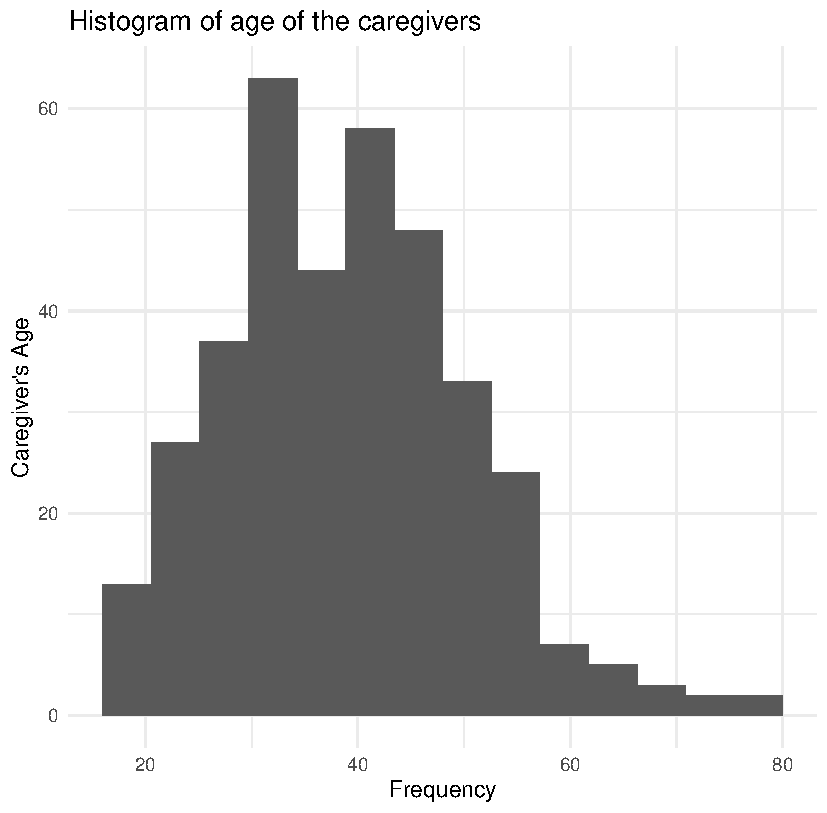
\includegraphics[width=\maxwidth]{Rplot01.pdf} 
\end{knitrout}

\begin{knitrout}
\definecolor{shadecolor}{rgb}{0.969, 0.969, 0.969}\color{fgcolor}\begin{kframe}
\begin{alltt}
\hlkwd{ggplot}\hlstd{(Data_care,}\hlkwd{aes}\hlstd{(age_pat),}\hlkwc{color}\hlstd{=}\hlstr{"blue"}\hlstd{)}\hlopt{+}
  \hlkwd{geom_histogram}\hlstd{(}\hlkwc{bins}\hlstd{=}\hlnum{10}\hlstd{)}\hlopt{+}
  \hlkwd{labs}\hlstd{(}\hlkwc{x}\hlstd{=}\hlstr{"frequency"}\hlstd{,}\hlkwc{y}\hlstd{=}\hlstr{"Patients age"}\hlstd{,}
       \hlkwc{title} \hlstd{=} \hlstr{"Histogram of age of patients"}\hlstd{)}\hlopt{+}
  \hlkwd{theme_minimal}\hlstd{()}
\end{alltt}
\end{kframe}
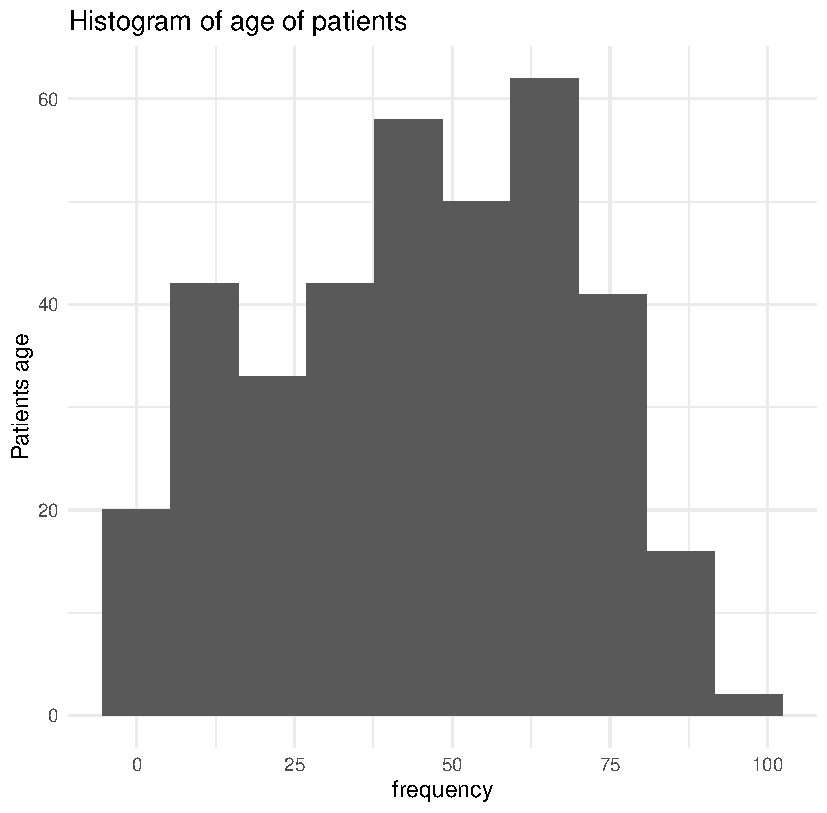
\includegraphics[width=\maxwidth]{Rplot02.pdf} 
\end{knitrout}

\subsubsection{Multivariate Normality}

Before we conduct multiple linear regression,we check if the data meets the assumptions of a multiple linear regression. One of the assumptions is the multivariate normality. To do this, we use the chi-square plot to plot the squared Mahalanobis distance to assess this assumption.

\begin{knitrout}
\definecolor{shadecolor}{rgb}{0.969, 0.969, 0.969}\color{fgcolor}\begin{kframe}
\begin{alltt}
\hlkwd{chisq.plot}\hlstd{(Data_care)}
\end{alltt}
\end{kframe}
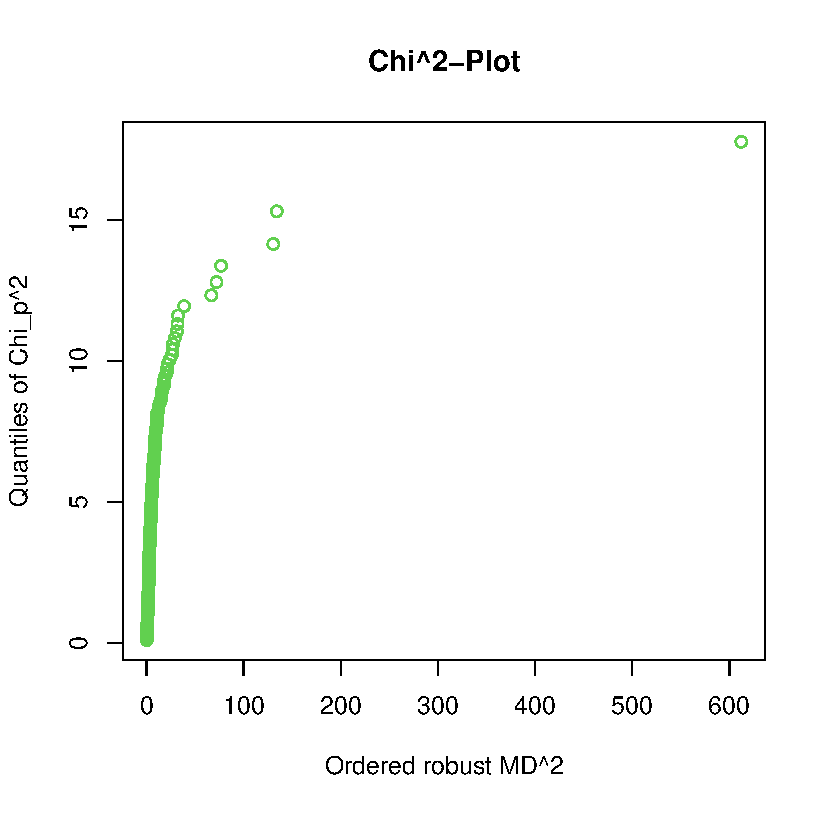
\includegraphics[width=\maxwidth]{Rplot03.pdf} 
\begin{kframe}\begin{verbatim}
## Remove outliers with left-click, stop with right-click on plotting device
## $outliers
## NULL
\end{verbatim}
\end{kframe}
\end{knitrout}
\noindent The data is not multivariate normal. Hence we normalize the data by taking natural log of the independent random variables to minimize on the effects f the outliers in the dataset.\\~\\

\textbf{Data Transformation}
\begin{knitrout}
\definecolor{shadecolor}{rgb}{0.969, 0.969, 0.969}\color{fgcolor}\begin{kframe}
\begin{alltt}
\hlstd{PHQ}\hlkwb{<-}\hlstd{Data_care}\hlopt{$}\hlstd{PHQ}
\hlstd{age_care}\hlkwb{<-}\hlkwd{log}\hlstd{(Data_care}\hlopt{$}\hlstd{age_care)}
\hlstd{age_pat}\hlkwb{<-}\hlkwd{log}\hlstd{(Data_care}\hlopt{$}\hlstd{age_pat)}
\hlstd{income}\hlkwb{<-}\hlkwd{log}\hlstd{(Data_care}\hlopt{$}\hlstd{income)}
\hlstd{data_trans}\hlkwb{<-}\hlkwd{cbind}\hlstd{(PHQ,age_care,age_pat,income)}
\hlkwd{View}\hlstd{(data_trans)}
\hlkwd{dim}\hlstd{(data_trans)}
\hlkwd{sum}\hlstd{(}\hlkwd{is.na}\hlstd{(data_trans))}
\hlkwd{sum}\hlstd{(}\hlkwd{is.infinite}\hlstd{(data_trans))}
\end{alltt}
\end{kframe}
\end{knitrout}



\noindent \textbf{Multivariate normality check of the transformed data}

\begin{knitrout}
\definecolor{shadecolor}{rgb}{0.969, 0.969, 0.969}\color{fgcolor}\begin{kframe}
\begin{alltt}
\hlkwd{pairs}\hlstd{(data_trans[,}\hlopt{-}\hlnum{1}\hlstd{])}
\end{alltt}
\end{kframe}
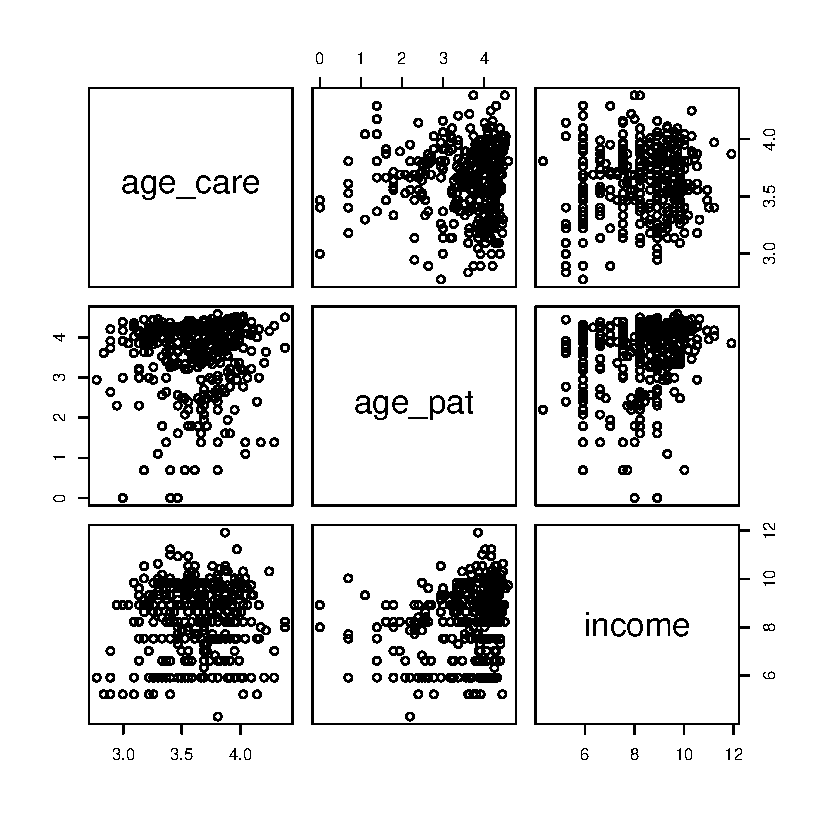
\includegraphics[width=\maxwidth]{Rplot04.pdf} 
\begin{kframe}\begin{alltt}
\hlkwd{chisq.plot}\hlstd{(data_trans)}
\end{alltt}
\end{kframe}
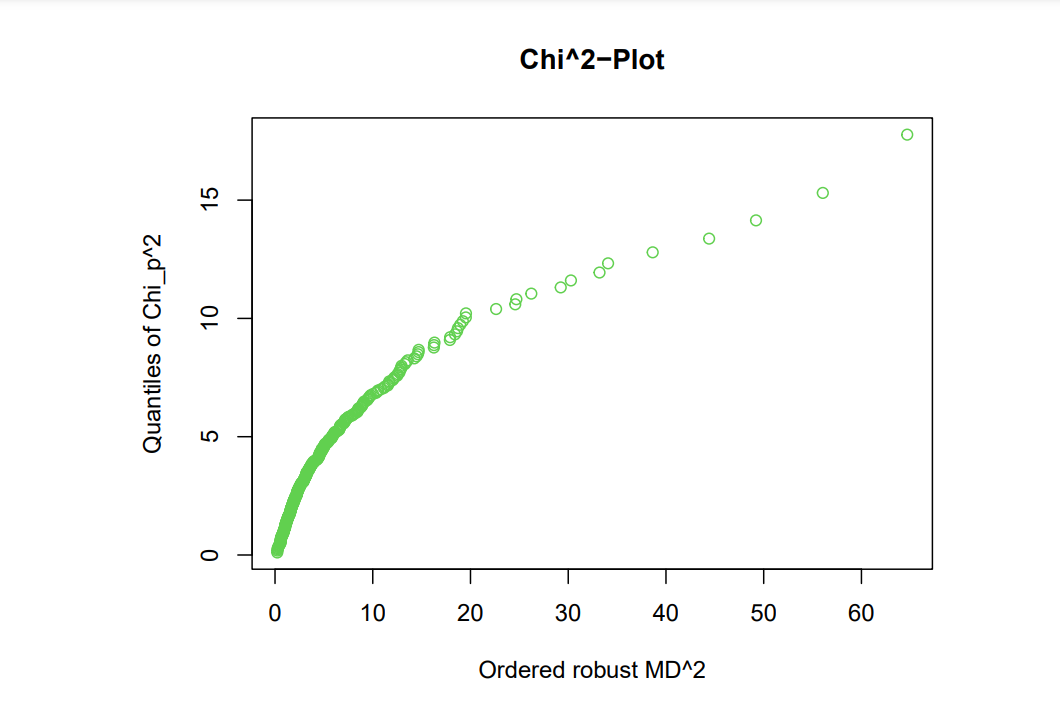
\includegraphics[width=\maxwidth]{Rplot05.png} 
\begin{kframe}\begin{verbatim}
## Remove outliers with left-click, stop with right-click on plotting device
## $outliers
## NULL
\end{verbatim}
\end{kframe}
\end{knitrout}
\noindent From the pairs plot, the data form ellipsoid clusters implying the data is multivariate normal as it is confirmed also by the squared Mahalanobis' distance plot.

\subsection{Multiple linear Regression model}
\begin{knitrout}
\definecolor{shadecolor}{rgb}{0.969, 0.969, 0.969}\color{fgcolor}\begin{kframe}
\begin{alltt}
\hlstd{data1}\hlkwb{<-}\hlkwd{as.data.frame}\hlstd{(data_trans)}
\hlstd{Model}\hlkwb{<-}\hlkwd{lm}\hlstd{(PHQ}\hlopt{~}\hlstd{age_care}\hlopt{+}\hlstd{age_pat}\hlopt{+}\hlstd{income,} \hlkwc{data} \hlstd{= data1)}
\hlkwd{summary}\hlstd{(Model)}
\end{alltt}
\begin{verbatim}
## 
## Call:
## lm(formula = PHQ ~ age_care + age_pat + income, data = data1)
## 
## Residuals:
##    Min     1Q Median     3Q    Max 
## -6.870 -2.466 -0.833  1.777 16.270 
## 
## Coefficients:
##             Estimate Std. Error t value Pr(>|t|)    
## (Intercept)  11.3014     2.3971   4.715 3.47e-06 ***
## age_care     -0.2735     0.5941  -0.460 0.645547    
## age_pat      -0.7151     0.2079  -3.440 0.000649 ***
## income       -0.4352     0.1286  -3.385 0.000791 ***
## ---
## Signif. codes:  0 '***' 0.001 '**' 0.01 '*' 0.05 '.' 0.1 ' ' 1
## 
## Residual standard error: 3.409 on 361 degrees of freedom
## Multiple R-squared:  0.07711,	Adjusted R-squared:  0.06944 
## F-statistic: 10.05 on 3 and 361 DF,  p-value: 2.23e-06
\end{verbatim}
\begin{alltt}
\hlcom{#anova(Model)}
\end{alltt}
\end{kframe}
\end{knitrout}

\noindent The model adopted  $\tilde{Y}=\beta_{0}+\beta_{i}log X$.\\
on the implied model, 1\% change in X leads to approximately $\beta_{i}$/100 unit change in Y.\\~\\

\noindent The estimated model is:
$\tilde{y}=11.3014-0.2735x_{1}-0.7151x_{2}-0.4352x_{3}$

\subsubsection{ANOVA table}
	\begin{tabular}{cccccc}
		\hline     
		Source of variation	& DF & SS &MS  &F  & Significance F \\
		\hline
		Regression	& 3 &350.5177596  & 116.8392532 &10.05417451	  &2.23044E-06  \\
		
		Residual	&	361  & 4195.169912	 &11.62096928	  &  &  \\
		
		Total	& 	364 & 4545.687671	 &  &  &  \\
		\hline
	\end{tabular}
	
\subsection{Data interpretation and Discussions}
We evaluate our model parameter estimates and do diagnostic tests for the model to assess the model fit.
\subsubsection{Model Evaluation}


\begin{knitrout}
\definecolor{shadecolor}{rgb}{0.969, 0.969, 0.969}\color{fgcolor}\begin{kframe}
\begin{verbatim}
## (Intercept)    age_care     age_pat      income 
##  11.3014112  -0.2734778  -0.7150504  -0.4352175
\end{verbatim}
\end{kframe}
\end{knitrout}
\noindent At 95\% significance, the intercept and age of the patient and income levels of the care givers are significant in determining the PHQ levels of the care giver. As noted, the age of the care giver is not significant in determining the PHQ levels of the care giver.\\~\\
1\% change in age of the care giver leads to approximately (-0.2734778 )/100 unit change in in the PHQ levels.\\
1\% change in age of the age of the patient leads to approximately (-0.7150504 )/100 unit change in in the PHQ levels.\\
1\% change in income  of the care giver leads to approximately ( -0.4352175 )/100 unit change in in the PHQ levels.\\~\\

\noindent The model's residual standard error is 3.409 on 361 degrees of freedom.Multiple R-squared is  0.07711 implying the model fit explains approximately 7\% variation in the data.	Adjusted R-squared is 0.06944.\\ 
F-statistic: 10.05 on 3 and 361 degrees of freedom at $\alpha$ - level =0.05 . The p-value 2.23e-06 suggests that there is strong evidence against the null hypothesis indicating that the model fit is statistically significant and is likely to have  a true relationship on the population of care givers we are studying.

\subsubsection{Diagnostics}

\textbf{i. Linearity}\\
We test that assumption that the model is linaer with respect to $\beta_{i} 's$
\begin{knitrout}
\definecolor{shadecolor}{rgb}{0.969, 0.969, 0.969}\color{fgcolor}\begin{kframe}
\begin{alltt}
\hlkwd{plot}\hlstd{(PHQ,age_care)}
\end{alltt}
\end{kframe}
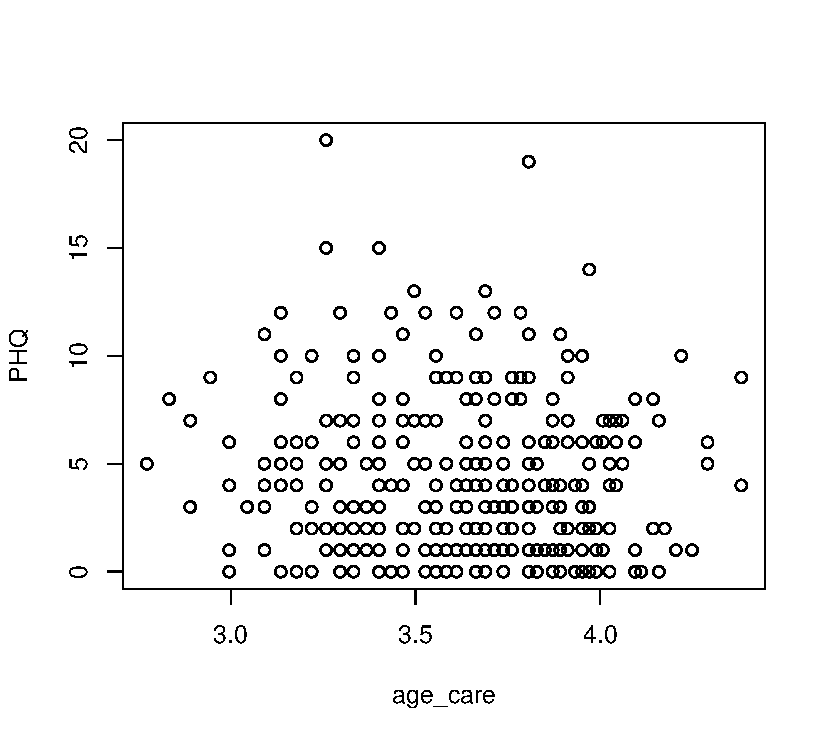
\includegraphics[width=\maxwidth]{Rplot06.pdf} 
\begin{kframe}\begin{alltt}
\hlkwd{plot}\hlstd{(PHQ,age_pat)}
\hlkwd{plot}\hlstd{(PHQ,age_pat)}
\end{alltt}
\end{kframe}
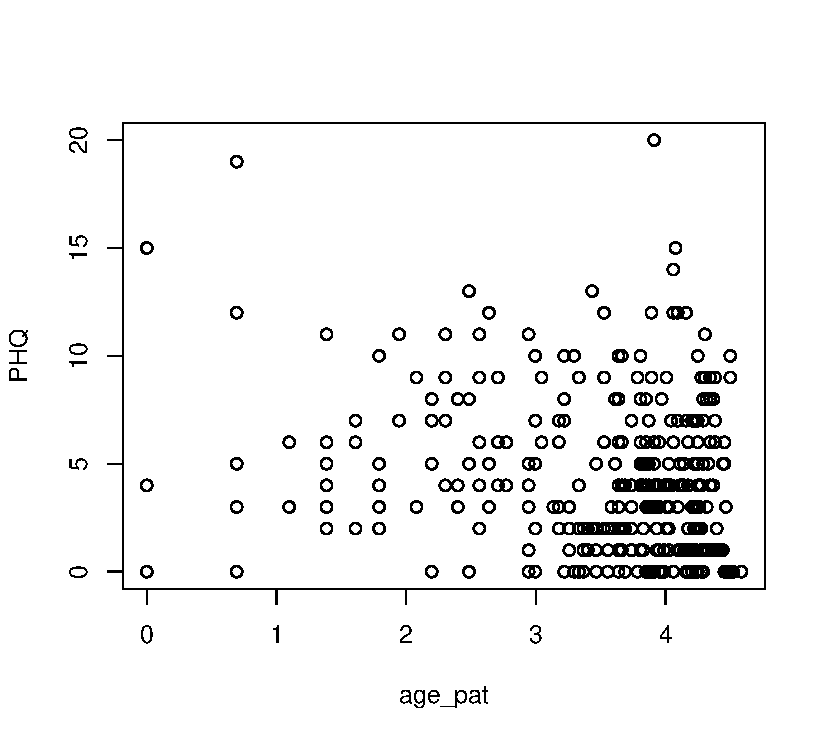
\includegraphics[width=\maxwidth]{Rplot07.pdf} 
\end{knitrout}

\noindent There is a linear relationship between the dependent variables and independent variables.\\~\\

\noindent \textbf{Normality of the residuals}
\begin{knitrout}
\definecolor{shadecolor}{rgb}{0.969, 0.969, 0.969}\color{fgcolor}\begin{kframe}
\begin{alltt}
\hlkwd{qqnorm}\hlstd{(}\hlkwd{residuals}\hlstd{(Model))}
\end{alltt}
\end{kframe}
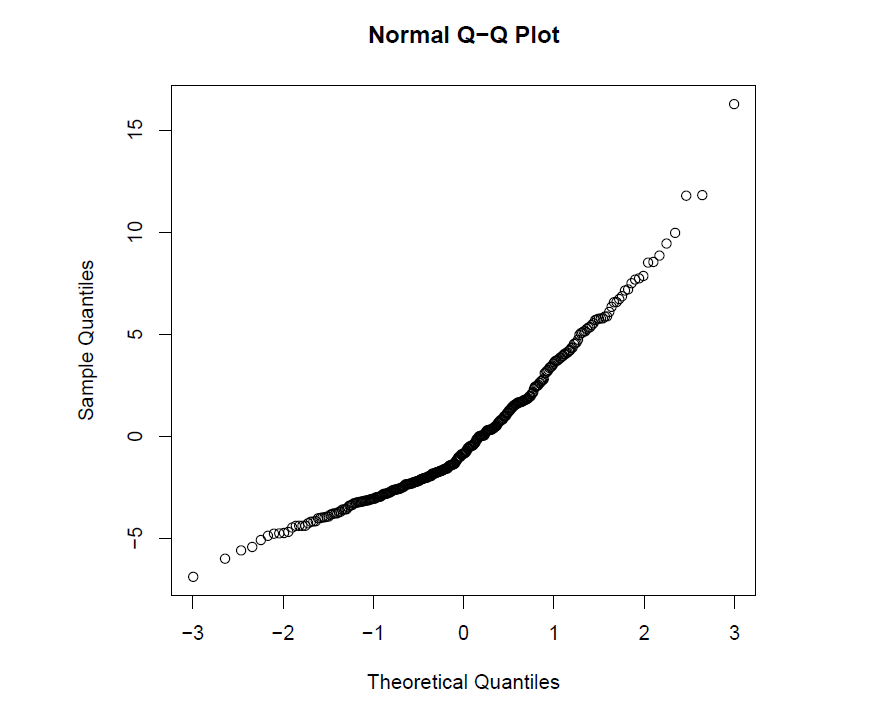
\includegraphics[width=\maxwidth]{Rplot09.png} 
\end{knitrout}
The qqnorm plot shows the residuals are normally distributed\\~\\

\noindent \textbf{ii.Homoscedasticity}
\begin{knitrout}
\definecolor{shadecolor}{rgb}{0.969, 0.969, 0.969}\color{fgcolor}\begin{kframe}
\begin{alltt}
\hlkwd{plot}\hlstd{(Model}\hlopt{}\hlstd{fitted.values,}\hlkwd{rstandard}\hlstd{(Model),}\hlkwc{ylab}\hlstd{=}\hlstr{"Standardised residuals"}\hlstd{)}
\end{alltt}
\end{kframe}

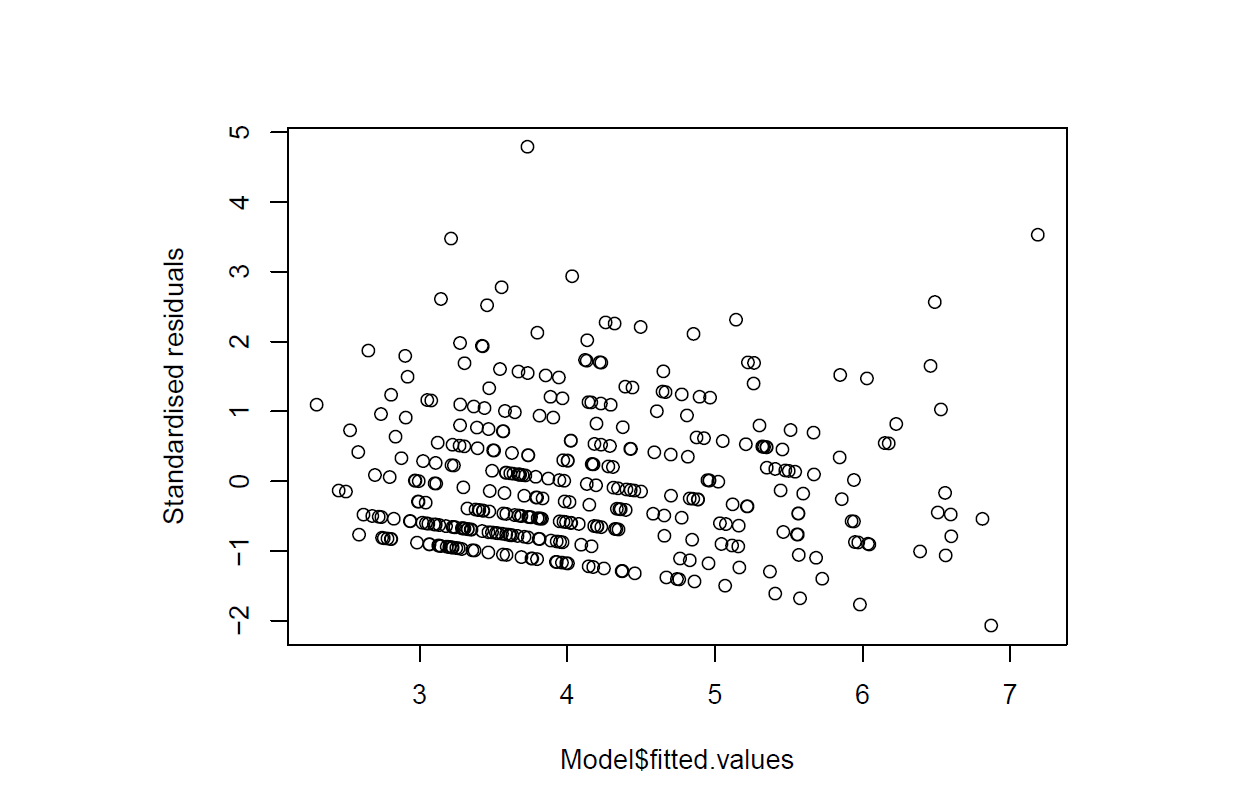
\includegraphics[width=\maxwidth]{Rplot10.png} 
\end{knitrout}
\noindent The variance of the the errors is constant across all the levels as evidenced by the plot above since the residuals have  a constant mean of zero\\~\\

\noindent \textbf{iii. Multi colinearity diagnostics}\\
\noindent Test of no multi-colinearity
\begin{knitrout}
\definecolor{shadecolor}{rgb}{0.969, 0.969, 0.969}\color{fgcolor}\begin{kframe}
\begin{alltt}
\hlkwd{library}\hlstd{(car)}
\hlkwd{vif}\hlstd{(Model)}
\end{alltt}
\begin{verbatim}
## age_care  age_pat   income 
## 1.003792 1.048467 1.052330
\end{verbatim}
\end{kframe}
\end{knitrout}
\noindent Each independent variable has a Variance inflation factor of 1 indicating no correlation between the independent variable and other variables in the model.\\~\\

\textbf{iv. Autocorrelation}
\begin{knitrout}
\definecolor{shadecolor}{rgb}{0.969, 0.969, 0.969}\color{fgcolor}\begin{kframe}
\begin{alltt}
\hlkwd{acf}\hlstd{(Model}\hlopt{}\hlstd{residuals)}
\end{alltt}
\end{kframe}
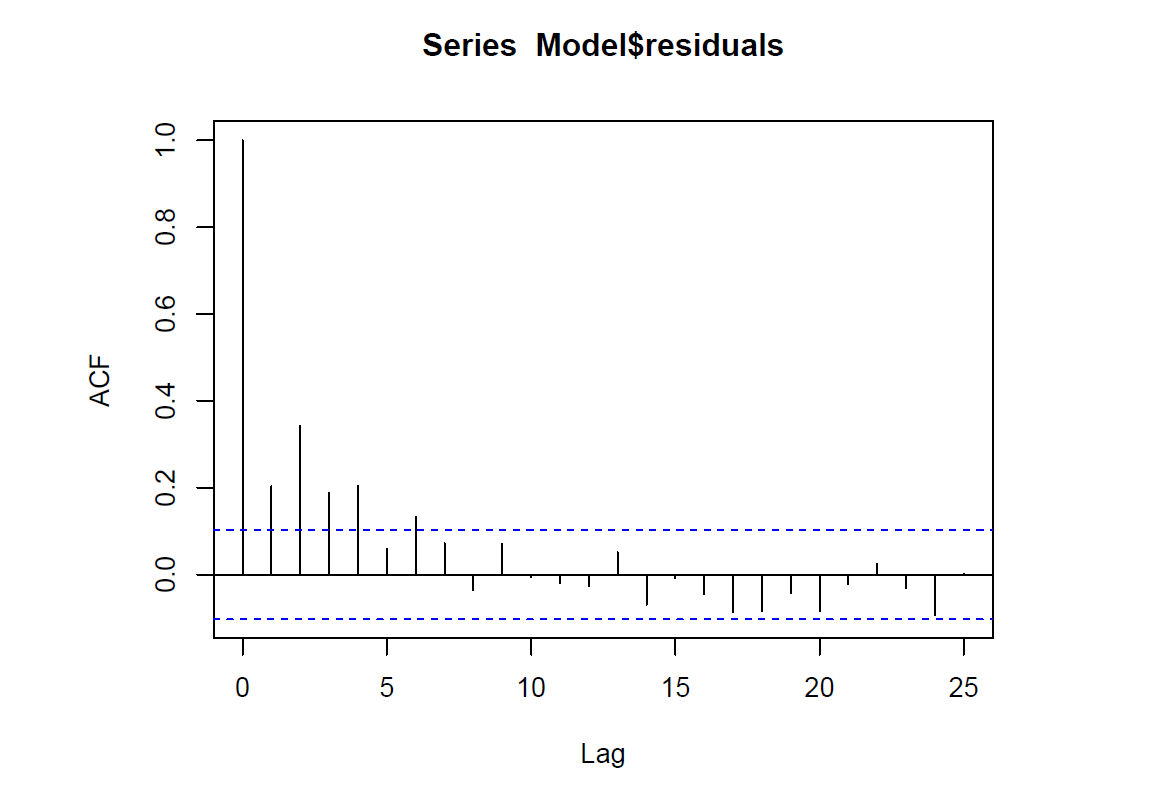
\includegraphics[width=\maxwidth]{Rplot11.png} 
\end{knitrout}
\noindent The residuals are independent of each other as shown by the ACF graph.
There is no significant auto-correlation. Hence the residuals are not independent of each other.
\newpage

	\section*{CHAPTER FIVE}
\section*{CONCLUSION}
\setcounter{section}{5}
\setcounter{subsection}{0}
\subsection{Introduction}
This research project utilized multiple linear regression analysis to investigate the relationships between the independent variables (age of patient, age of participant, and level of income) and the dependent variable (level of depression) among caregivers in rural settings. The findings of this study contribute to our understanding of the factors influencing depression among these individuals and have the potential to inform the development of targeted interventions to support their mental well-being. By identifying predictors, measuring associations, examining interactions, evaluating model performance, and offering evidence-based suggestions for interventions, this research offers valuable insights for addressing depression among cancer caregivers in rural settings.
\subsection{Summary}
This research project examines the relationships between independent variables (age of patient, age of participant, and level of income) and the dependent variable (level of depression) among caregivers in rural settings. By conducting multiple linear regression, the study has identified predictors and understanding of the factors influencing depression in this population. The findings will contribute to our understanding of depression among rural caregivers, informing the development of targeted interventions and providing evidence-based suggestions to support their mental health.
\subsection{Conclusions}
This research project utilized multiple linear regression analysis to investigate the relationships between independent variables (age of patient, age of participant, and level of income) and the dependent variable (level of depression) among caregivers in rural settings. The findings of this study have contributed significantly to our understanding of the factors that influence depression among these individuals and can provide valuable insights for the development of targeted interventions.\\

\noindent By identifying predictors, measuring associations, examining interactions, and evaluating model performance, this research has provided a comprehensive examination of the factors associated with depression among cancer caregivers in rural settings. The evidence-based suggestions derived from these findings can inform the development of interventions specifically tailored to address the unique challenges faced by these individuals.\\

\noindent The outcomes of this study have practical implications for supporting caregivers in rural areas who experience depression. By understanding the factors influencing depression in this context, interventions can be designed to address these factors and provide effective support. This research contributes to the growing body of knowledge on mental health in caregiving situations and highlights the importance of considering the specific needs of caregivers in rural settings.\\

\noindent The rigorous analysis conducted in this project enhances the reliability and validity of the findings. By employing multiple linear regression, the relationships between variables have been thoroughly examined, providing valuable insights into the complex dynamics involved in depression among caregivers in rural settings.\\

\noindent Overall, the results of this study have the potential to make a meaningful impact on the well-being of caregivers in rural areas by informing the development of evidence-based interventions. By addressing the factors identified in this research, interventions can be tailored to meet the specific needs of these caregivers, ultimately improving their mental health outcomes and overall quality of life.
\newpage
\subsection{Recommendation}
Based on the findings of this research project, several evidence-based recommendations can be made to inform the development of targeted interventions for depression among cancer caregivers in rural settings:\\
\begin{enumerate}
	\item Develop tailored support programs: Based on the identified predictors and factors influencing depression, it is crucial to design interventions specifically tailored to the needs of caregivers in rural areas. These programs should consider the unique challenges faced by this population, such as limited access to resources, social isolation, and financial constraints.\\
	
	\item Incorporate age-specific interventions: Given the significance of age in the regression analysis, interventions should be designed to address the varying needs and experiences of caregivers of different age groups. For instance, younger caregivers may require assistance with balancing caregiving responsibilities and personal development, while older caregivers may need support with physical health and age-related concerns.\\
	
	\item Enhance social support networks: Social isolation can contribute to depression among caregivers in rural settings. Interventions should focus on strengthening social support networks by connecting caregivers with support groups, local community resources, and online platforms. Peer support and opportunities for shared experiences can help alleviate feelings of isolation and provide emotional support.\\  
	
	\item Provide financial assistance and resources: The level of income emerged as an important factor in the regression analysis. Interventions should address the financial challenges faced by caregivers in rural areas, such as limited job opportunities or transportation costs. Offering financial assistance programs or connecting caregivers with available resources can help alleviate financial stress and improve their mental well-being.\\
	
	\item Implement caregiver education and training: Providing caregivers with educational resources and training can equip them with the necessary skills to navigate the challenges of caregiving effectively. Workshops or online modules can focus on stress management, self-care practices, communication skills, and strategies for coping with the emotional demands of caregiving.\\
	
	
\end{enumerate}

\newpage
\section*{REFERENCES}
\begin{enumerate}
	\item Jain G., Roy A., Harikrishnan V., Yu S., Dabbous O. and Lawrence, C. (2013), Patient-Reported Depression Severity Measured by the PHQ-9 and Impact on Work Productivity, \emph{Journal of Occupational and Environmental Medicine}, 55(3), 252-258.
	
	\item Laing S. S., and Jones S. M. (2016), Anxiety and Depression Mediate the Relationship between Perceived Workplace Health Support and Presenteeism, \emph{Journal of Occupational and Environmental Medicine}, 58(11), 1144-1149.
	
	\item Leung D. Y., Mak Y. W., Leung S. F., Chiang V. C. and Loke A. Y. (2020), Measurement Invariances of the PHQ‐9 Across Gender and Age Groups in Chinese Adolescents,\emph{ Asia‐Pacific Psychiatry}, 12(3), e12381.
	
	\item Levis B., Benedetti A. and Thombs B. D. (2019), Accuracy of Patient Health Questionnaire-9 (PHQ-9) For Screening to Detect Major Depression: Individual Participant Data Meta-Analysis,\emph{BMJ}, 365.
	
	\item Levis B., Sun Y., He C., Wu Y., Krishnan A., Bhandari P. M. and Thombs B. D. (2020), Accuracy of the PHQ-2 Alone and in Combination with the PHQ-9 for Screening to Detect Major Depression: Systematic Review and Meta-Analysis,\emph{ JAMA}, 323(22), 2290-2300.
	
	\item Lister K., Seale J. and Douce C. (2023), Mental Health in Distance Learning: A Taxonomy of Barriers and Enablers to Student Mental Wellbeing, \emph{Open Learning: The Journal of Open, Distance and e-Learning}, 38(2), 102-116.
	\item Kaggwa M. M., Najjuka, S. M., Nuwamanya S., Nabulo, H., and Nkola R. (2021). Depression among cancer caregivers in a rural setting.xlsx. Retrieved from
	\href{https://figshare.com/articles/dataset/Depressionamongcancercaregiversinaruralsettingxlsx/doi: 10.6084/m9.figshare.14524800.v1}{figshare}
	
	\item Magtibay D. L., Chesak S. S., Coughlin K. and Sood, A. (2017), Decreasing Stress and Burnout in Nurses, \emph{The Journal of Nursing Administration}, 47(7/8), 391-395.
	
	\item Martin A., Sanderson K. and Cocker F. (2009), Meta-Analysis of the Effects of Health Promotion Intervention in the Workplace on Depression and Anxiety Symptoms,\emph{Scandinavian Journal of Work, Environment and Health}, 7-18.
	\item  Montgomery C. D, Peck A. E and Vining G.G.(2012), Introduction to linear regression analysis, John Wiley \& Sons Inc.
	\item Serpa J. G., Taylor S. L. and Tillisch K. (2014), Mindfulness-Based Stress Reduction (MBSR) Reduces Anxiety, Depression, and Suicidal Ideation in Veterans, \emph{Medical Care}, 52(12), S19-S24.
\end{enumerate}

\end{document}

